\part{Oscillations and Waves}
\chapter{Single oscillator}
\section{Harmonic oscillation}
\vocab{Restoring force or torque} is the resultant force or torque directed towards the equilibrium position.

\vocab{Simple harmonic motion}: restoring force or torque is linear, i.e. net force is directed towards the equilibrium position and is proportional to displacement from equilibrium.

\subsection{Kinematics and Energy}
Frequency and period are related by
\begin{equation}
f=\frac{1}{T}
\end{equation}

Angular frequency, frequency and period are related by
\begin{equation}
\omega = 2\pi f = \frac{2\pi}{T}
\end{equation}

\textbf{Displacement}:
\begin{equation}
{x(t)=A\cos\brac{\omega t+\phi_0}
}\end{equation}
where $A$ and $\phi_0$ are constants determined by initial conditions $x$ ($t=0$) and $v_x$ ($t=0$).
\begin{proof}[Derivation]
By Newton's 2nd Law,
\[ F_x=-kx_x=ma_x \implies a_x=-\frac{k}{m}x \implies \dv[2]{x(t)}{t}=-\frac{k}{m}x(t)=-\omega^2x(t) \]
which is a second-order ordinary differential equation.
\end{proof}

\textbf{Velocity}:
\begin{equation}
{v_x(t)=\dv{x(t)}{t}=-\omega A\sin(\omega t+\phi_0)
}\end{equation}

\textbf{Acceleration}:
\begin{equation}
{a_x(t)=\dv{v_x(t)}{t}=-\omega^2 A\cos(\omega t+\phi_0)
}\end{equation}

\textbf{Kinetic energy}:
\begin{equation}
{K(t)=\frac{1}{2}mv_x(t)^2=\frac{1}{2}m\omega^2A^2\sin^2\brac{\omega t+\phi_0}
}\end{equation}

\textbf{Potential energy}:
\begin{equation}
{U(t)=\frac{1}{2}kx(t)^2=\frac{1}{2}kA^2\cos^2\brac{\omega t+\phi_0}
}\end{equation}

Total energy is the sum of KE and PE:
\begin{equation}
{E(t)=K(t)+U(t)=\frac{1}{2}kA^2
}\end{equation}

\subsection{Newton’s Approach}
Consider a spring-mass system, as shown below:
\begin{figure}[H]
    \centering
    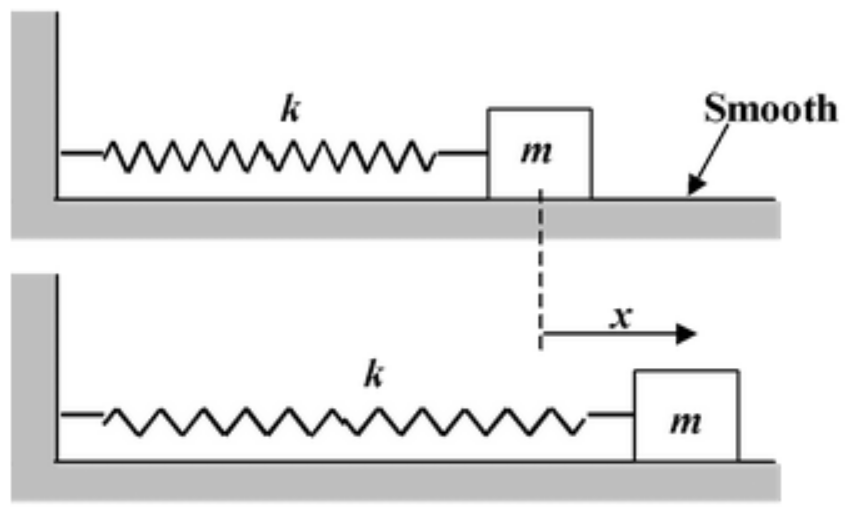
\includegraphics[width=8cm]{images/spring_mass_system.png}
\end{figure}

By Newton's 2nd Law, 
\begin{align*}
\sum\vb{F}(t) &= m\vb{a}(t) \\
-kx(t) &= m\dv[2]{x(t)}{t} \\
\dv[2]{x(t)}{t} &= -\frac{k}{m}x(t)
\end{align*}
where $\dfrac{k}{m}$ is a constant.

We define
\[ \omega^2 \equiv \frac{k}{m} \]

Then \[ \dv[2]{x(t)}{t} = -\omega^2x(t) \]

This 2nd order differential equation has the general solution for the \textbf{displacement function}:
\[ x(t)=A\cos\omega t + B\sin\omega t \]
where constants $A$ and $B$ are determined by the initial conditions, such as $x(0)=0$, $v(0)=v_0$. This gives us $A=x_0$ and $B=\frac{v_0}{\omega}$. 

Hence we have the displacement function for a particular oscillation:
\[ \boxed{x(t)=x_0\cos\omega t + \frac{v_0}{\omega}\sin\omega t} \]

Considering the period $T$, since the displacement function is periodic, we have $x(t)=x(t+T)$. Plugging this into the displacement function above, we have 
\begin{align*}
\cos(\omega t) &= \cos(\omega t+\omega T) \\
\cos(\omega t) &= \cos(\omega t+\omega T)
\end{align*}
The property of the sine and cosine functions gives us \[ \omega T=2\pi \implies \omega=\frac{2\pi}{T} \text{ and } \omega=2\pi f \]

This gives us \[ T=2\pi\sqrt{\frac{m}{k}} \]
\pagebreak

Using \textbf{simple pendulum motion} as another example, 

\begin{figure}[H]
    \centering
    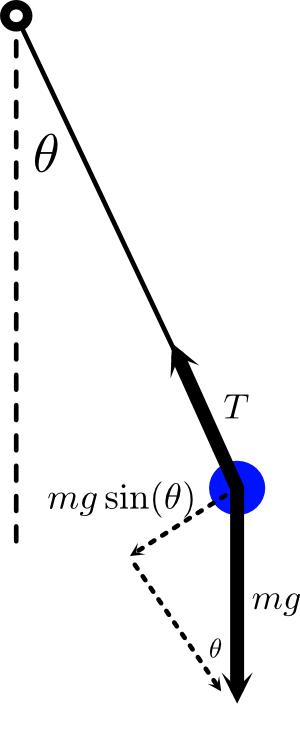
\includegraphics[width=4cm]{images/pendulum-fbd.png}
\end{figure}

By Newton's 2nd Law, 
\[ \vb{F}_t=m\vb{a}_t \implies -mg\sin\theta(t)=m\dv[2]{s(t)}{t} \]
By small angle approximation, $\sin\theta \approx \theta$.
\[ \dv[2]{\theta(t)}{t} = -\frac{g}{L}\sin\theta(t) \implies \dv[2]{\theta(t)}{t} \approx \frac{g}{L}\sin\theta(t) \equiv -\omega^2\theta(t) \]
Period of the motion:
\[ T=\frac{2\pi}{\omega}=2\pi\sqrt{\frac{L}{g}} \]
\pagebreak

For the \textbf{physical pendulum motion}, an \textbf{extended object} swings back and forth on a pivot under the influence of gravity.

\begin{figure}[H]
    \centering
    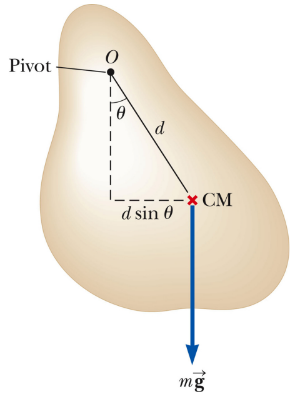
\includegraphics[width=6cm]{images/physical_pendulum.png}
\end{figure}

Net torque with respect to the pivot, using $\tau = I\alpha$:
\[ -mgd\sin\theta(t)=I\dv[2]{\theta(t)}{t} \implies \dv[2]{\theta(t)}{t}=-\frac{mgd}{I}\sin\theta(t) \]
By small approximation, $\sin\theta \approx \theta$
\[ \dv[2]{\theta(t)}{t} = -\frac{mgd}{I}\theta(t) \equiv -\omega^2\theta(t) \]
Hence period of the motion is given by
\[ T=\frac{2\pi}{\omega}=2\pi\sqrt{\frac{I}{mgd}} \]

\subsection{Energy conservation}
Using the above example of the simple pendulum motion, we analyse the energy of the pendulum.
\begin{align*}
E(t) &= \text{Rotational KE} + \text{GPE} \\
&= \frac{1}{2}I\omega^2 + mgL(1-\cos\theta(t)) \\
&= \frac{1}{2}(mL^2)\sqbrac{\dv{\theta(t)}{t}}^2 + mgL(1-\cos\theta(t)) \\
\dv{E(t)}{t} &= mL^2\dv{\theta(t)}{t}\dv[2]{\theta(t)}{t} + mgL\sin\theta(t)\dv{\theta(t)}{t}
\end{align*}

Since energy is conserved, total energy remains constant, hence
\[ \dv{E(t)}{t}=0 \implies L\dv[2]{\theta}{t} + g\sin\theta(t) = 0 \implies \dv[2]{\theta}{t}=-\frac{g}{L}\sin\theta(t) \]
and the rest follows.
\pagebreak

\begin{exmp}
A mass $M$ is connected to two springs 1, 2 of spring constants $k_1$ and $k_2$ and slides on a smooth horizontal table. In the equilibrium position it is given a velocity $v_0$ towards spring 2.
\begin{enumerate}[label=(\alph*)]
\item Find the period of the motion.
\item Find the amplitude of the motion.
\end{enumerate}
\end{exmp}

\begin{figure}[H]
    \centering
    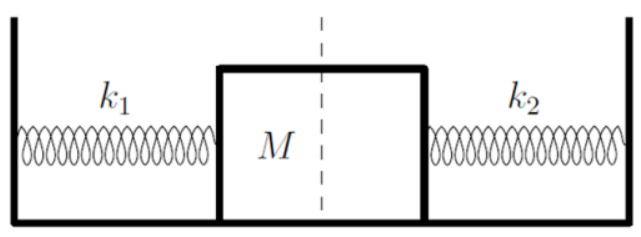
\includegraphics[width=6cm]{images/two_springs.png}
\end{figure}

\begin{proof}[Solution]
By Newton's 2nd Law,
\[ \sum\vb{F}(t)=-(k_1+k_2)x(t) \implies \dv[2]{x}{t}=-\frac{k_1+k_2}{M}x \implies \omega^2\equiv\frac{k_1+k_2}{M} \]
Period:
\[ \boxed{T=\frac{2\pi}{\omega}=2\pi\sqrt{\frac{M}{k_1+k_2}}} \]

By conservation of energy, loss in kinetic energy is converted to gain in elastic potential energy.
\[ \frac{1}{2}m{v_0}^2 = \frac{1}{2}k_1{x_0}^2 + \frac{1}{2}k_2{x_0}^2 \implies \boxed{x_0 = \sqrt{\frac{m{v_0}^2}{k_1+k_2}}} \]
\end{proof}
\pagebreak

\section{Damped oscillations}
Exponential decay of damped oscillations

\section{Forced oscillations and resonance}
resonance of sinusoidally forced oscillators: amplitude and phase shift of steady state oscillations. 

Free oscillations of LC-circuits; mechano-electrical analogy; positive feedback as a source of instability; generation of sine waves by feedback in a LC-resonator.


\chapter{Waves}
\section{Basics}
Propagation of harmonic waves: phase as a linear function of space and time; wave length, wave vector, phase and group velocities; exponential decay for waves propagating in dissipative media; transverse and longitudinal waves; the classical Doppler effect.

\section{Waves in inhomogeneous media}
Fermat’s principle, Snell’s law.

\section{Sound waves}
speed as a function of pressure (Young’s or bulk modulus) and density, Mach cone.

\section{Energy}
Energy carried by waves: proportionality to the square of the amplitude, continuity of the energy flux.
\pagebreak

\chapter{Interference and diffraction}
\section{Interference}
Superposition of waves: coherence, beats, standing waves, Huygens’ principle, interference due to thin films (conditions for intensity minima and maxima only).

\section{Diffraction}
Diffraction from one and two slits, diffraction grating, Bragg reflection.
\pagebreak

\chapter{Interaction of electromagnetic waves with matter}
Dependence of electric permittivity on frequency (qual-
itatively); refractive index; dispersion and dissipation of
electromagnetic waves in transparent and opaque ma-
terials. Linear polarisation; Brewster angle; polarisers;
Malus’ law.
\pagebreak

\chapter{Light and Optics}
\section{}

Approximation of geometrical optics: rays and optical images; a partial shadow and full shadow. 
Thin lens approximation; construction of images created by ideal thin lenses; thin lens equation.
Luminous flux and its continuity; illuminance; luminous intensity.
\pagebreak

\chapter{Optical devices}
Telescopes and microscopes: magnification and resolv-
ing power; diffraction grating and its resolving power;
interferometers.

\chapter{Relativity}
Principle of relativity and Lorentz transformations for
the time and spatial coordinate, and for the energy and
momentum; mass-energy equivalence; invariance of the
spacetime interval and of the rest mass. Addition of par-
allel velocities; time dilation; length contraction; relativ-
ity of simultaneity; energy and momentum of photons
and relativistic Doppler effect; relativistic equation of
motion; conservation of energy and momentum for elas-
tic and non-elastic interaction of particles.



